\documentclass{article}\usepackage[]{graphicx}\usepackage[]{color}
% maxwidth is the original width if it is less than linewidth
% otherwise use linewidth (to make sure the graphics do not exceed the margin)
\makeatletter
\def\maxwidth{ %
  \ifdim\Gin@nat@width>\linewidth
    \linewidth
  \else
    \Gin@nat@width
  \fi
}
\makeatother

\definecolor{fgcolor}{rgb}{0.345, 0.345, 0.345}
\newcommand{\hlnum}[1]{\textcolor[rgb]{0.686,0.059,0.569}{#1}}%
\newcommand{\hlstr}[1]{\textcolor[rgb]{0.192,0.494,0.8}{#1}}%
\newcommand{\hlcom}[1]{\textcolor[rgb]{0.678,0.584,0.686}{\textit{#1}}}%
\newcommand{\hlopt}[1]{\textcolor[rgb]{0,0,0}{#1}}%
\newcommand{\hlstd}[1]{\textcolor[rgb]{0.345,0.345,0.345}{#1}}%
\newcommand{\hlkwa}[1]{\textcolor[rgb]{0.161,0.373,0.58}{\textbf{#1}}}%
\newcommand{\hlkwb}[1]{\textcolor[rgb]{0.69,0.353,0.396}{#1}}%
\newcommand{\hlkwc}[1]{\textcolor[rgb]{0.333,0.667,0.333}{#1}}%
\newcommand{\hlkwd}[1]{\textcolor[rgb]{0.737,0.353,0.396}{\textbf{#1}}}%
\let\hlipl\hlkwb

\usepackage{framed}
\makeatletter
\newenvironment{kframe}{%
 \def\at@end@of@kframe{}%
 \ifinner\ifhmode%
  \def\at@end@of@kframe{\end{minipage}}%
  \begin{minipage}{\columnwidth}%
 \fi\fi%
 \def\FrameCommand##1{\hskip\@totalleftmargin \hskip-\fboxsep
 \colorbox{shadecolor}{##1}\hskip-\fboxsep
     % There is no \\@totalrightmargin, so:
     \hskip-\linewidth \hskip-\@totalleftmargin \hskip\columnwidth}%
 \MakeFramed {\advance\hsize-\width
   \@totalleftmargin\z@ \linewidth\hsize
   \@setminipage}}%
 {\par\unskip\endMakeFramed%
 \at@end@of@kframe}
\makeatother

\definecolor{shadecolor}{rgb}{.97, .97, .97}
\definecolor{messagecolor}{rgb}{0, 0, 0}
\definecolor{warningcolor}{rgb}{1, 0, 1}
\definecolor{errorcolor}{rgb}{1, 0, 0}
\newenvironment{knitrout}{}{} % an empty environment to be redefined in TeX

\usepackage{alltt}
\usepackage{longtable}
\usepackage{geometry}
\usepackage[round]{natbib}
% \usepackage{natbib}
\bibliographystyle{abbrvnat}
\usepackage{graphicx}
\geometry{a4paper}
\usepackage[T1]{fontenc}
\usepackage[utf8]{inputenc}
\usepackage{authblk}
\usepackage[running]{lineno}
\usepackage{setspace}
\usepackage{courier}
% \usepackage{tabulary}
\usepackage{hyperref}
\doublespacing
\IfFileExists{upquote.sty}{\usepackage{upquote}}{}
\begin{document}
\linenumbers

\newpage

\section*{Appendix S1: Pre-processing \texttt{popler} data}
Before uploading datasets into the online \texttt{popler} database, we combined datasets, transformed datasets from wide to long form, converted non-ASCII characters, and modified ambiguous study site names.

The variables of many datasets were contained in two or more separate files, which we combined in a single file. When the original dataset provided data in wide form, we transformed it into long form. In wide form datasets, abundance data associated with different species was stored in separate columns. \texttt{popler} stores these datasets in long form, whereby each row of abundance data is related to a specific taxonomic unit in the table containing taxonomic information (Fig. \ref{Fig:schema}B). We converted all data in ASCII format, because the encoding of the database is the UTF-8. We often re-defined study site names to unambiguously associate them with one of the 26 LTER sites. Many site names are alphanumeric codes (e.g. ``U1'') which can overlap across several LTER sites. Hence, we changed site names following a standard formula (namely, from ``U1'' to ``site\textunderscore sbc\textunderscore U1'', where ``sbc'' refers to the Santa Barbara coastal LTER site).

In a handful of cases, we removed single data rows from the original dataset. These data rows were associated with two types of typos in the original dataset. First, some abundance observations were not associated with a time of observation. We removed this data because \texttt{popler} can only accommodate population information associated with a time of observation. Second, a handful of abundance data points were clear typos (e.g. the letter ``l'' instead of a numeric value). We substituted these data points with a missing value. We uploaded these pre-processed datasets in the \texttt{popler} database through a Graphic User Interface developed in Python using libraries panda and pyqt5.

\newpage
\setcounter{table}{0}
\renewcommand{\thetable}{S\arabic{table}}

 \begin{table}[h!]
%\begin{longtable}{p{10cm} p{5cm}}
  \caption{Taxonomic variables contained in the popler table on original taxonomic information.}
  \label{Tab:S1}
   \begin{center}
     \begin{tabular}{l}
      \hline
      Variable\\
      \hline
      \texttt{sppcode} \\
      \texttt{kingdom}\\
      \texttt{subkingdom}\\
      \texttt{infrakingdom}\\
      \texttt{superdivision}\\
      \texttt{division}\\
      \texttt{subdivision}\\
      \texttt{superphylum}\\
      \texttt{phylum}\\
      \texttt{subphylum}\\
      \texttt{class}\\
      \texttt{subclass}\\
      \texttt{order}\\
      \texttt{family}\\
      \texttt{genus}\\
      \texttt{species}\\
      \texttt{common\textunderscore name}\\
      \hline
     \end{tabular}
   \end{center}
 \end{table}
%\end{longtable}

\newpage
 %\begin{table}[h!]
   %\caption{Metadata variables used to describe the datasets stored in \texttt{popler.}}
   %\label{Tab:S2}
   %\begin{center}
   %\begin{tabular}{p{10cm} p{5cm}}
    \begin{longtable}{p{10cm} p{5cm}}
      \caption{Metadata variables used to describe the datasets stored in \texttt{popler.}}
      \label{Tab:S2}\\
      \hline
      Variable & Description \\
      \hline
\texttt{proj\textunderscore metadat\textunderscore key} & {Unique ID} \\
\texttt{lter\textunderscore project\textunderscore key} & {ID of LTER site} \\
\texttt{lter\textunderscore project\textunderscore key} & {ID of LTER site} \\
\texttt{title} & {Title of study} \\
\texttt{samplingunits} & {Unit of measure (if any) referred to population data.} \\
\texttt{datatype} & {Data type: count, biomass, cover, density, and individual. These correspond to the tables in Fig. 1A.} \\
\texttt{structured\textunderscore data} & {If data type is not individual, but the abundance observations refer to sub-groups of the population based on, for example, sex, developmental stage, or age)} \\
\texttt{structured\textunderscore type\textunderscore n} & {If individual data, this shows what type of structure is stored. A study can contain up to $n = 4$ types of structure.}\\
\texttt{structured\textunderscore type\textunderscore n\textunderscore units} & {Unit of measure (if any) referred to structure data.}\\
\texttt{studystartyr} & {Start year of the study} \\
\texttt{studyendyr} & {End year of the study} \\
\texttt{duration\textunderscore years} & {Duration of the study in years} \\
\texttt{samplefreq} & {Frequency of population census} \\
\texttt{studytype} & {Whether study is observational or experimental} \\
\texttt{community} & {Whether study includes single taxon (\texttt{community = F}) or multiple taxa (\texttt{community = T})} \\
\texttt{spatial\textunderscore replication\textunderscore level\textunderscore n\textunderscore extent} & {Extent of spatial replication level number $n$. A dataset can have up to 5 replication levels.} \\
\texttt{spatial\textunderscore replication\textunderscore level\textunderscore n\textunderscore extent\textunderscore units} & {Unit of spatial extent of the $n$ spatial replication level.} \\
\texttt{spatial\textunderscore replication\textunderscore level\textunderscore n\textunderscore label} & {Label of the spatial replication level (e.g. transect, plot, quadrat, ect.). The label of spatial replication level 1 is ``site''.} \\
\texttt{spatial\textunderscore replication\textunderscore level\textunderscore n\textunderscore number\textunderscore of\textunderscore unique\textunderscore reps} & {The number of unique replicates for the $n$th level of spatial replication.} \\
\texttt{treatment\textunderscore type\textunderscore n} & {The type of treatment (e.g. resource manipulation). A study can contain up to \texttt{n = 3} treatments.} \\
\texttt{control\textunderscore group} & {If study is experimental, this shows the field(s) that identify the control replicate.} \\
\texttt{derived} & {Is population size data raw, or is it derived (e.g. it is aggregated)?} \\
\texttt{authors} & {Author(s) of the original dataset} \\
\texttt{authors\textunderscore contact} & {Email address(es) of the author(s) associated with the original dataset.} \\
\texttt{metalink} & {url of the original dataset} \\
\texttt{knbid} & {Knowledge Network for Biocomplexity identifier.} \\
\texttt{doi} & {Digital object identifier of the original dataset} \\
      \hline
    \end{longtable}
    %\end{tabular}
   %\end{center}
 %\end{table}     
     
\newpage     
 \begin{table}[h!]
%\begin{longtable}{p{10cm} p{5cm}}
  \caption{LTER identification acronyms and their meaning as used in the \texttt{popler} database.}
  \label{Tab:S3}
   \begin{center}
     \begin{tabular}{l l}
      \hline
      Variable & LTER name\\
      \hline
AND & Andrew Forest LTER \\                        
ARC & Arctic LTER \\                               
BES & Baltimore Ecosystem Study \\                 
BNZ & Bonanza Creek LTER \\                        
CAP & Central Arizona - Phoneix LTER \\            
CCE & California Current Ecosystem LTER \\         
CDR & Cedar Creek Ecosystem Science Reserve LTER \\
CWT & Coweeta LTER \\                              
FCE & Florida Coastal Everglades LTER \\           
GCE & Georgia Coastal Ecosystems LTER \\           
HBR & Hubbard Brook LTER \\                        
HFR & Harvard Forest LTER \\                       
JRN & Jornada Basin LTER \\                        
KBS & Kellogg Biological Station LTER \\           
KNZ & Konza Prairie LTER \\                        
LNO & LTER Network Office \\                       
LUQ & Luquillo LTER \\                             
MCM & McMurdo Dry Valleys LTER \\                  
MCR & Moorea Coral Reef LTER \\                    
NCO & LTER Network Communications Office \\        
NTL & North Temperate Lakes LTER \\                
NWT & Niwot Ridge LTER \\                          
PAL & Palmer Antarctica LTER \\                    
PIE & Plum Island Ecosystems LTER \\               
SBC & Santa Barbara Coastal LTER \\                
SEV & Sevilleta LTER  \\                           
SGS & Shortgrass Steppe LTER \\                    
VCR & Virginia Coastal Reserve LTER \\
      \hline
     \end{tabular}
   \end{center}
 \end{table}
%\end{longtable}

\setcounter{figure}{0}
\renewcommand{\thefigure}{S\arabic{figure}}

\newpage
\begin{figure}[h!]
  \begin{center}
    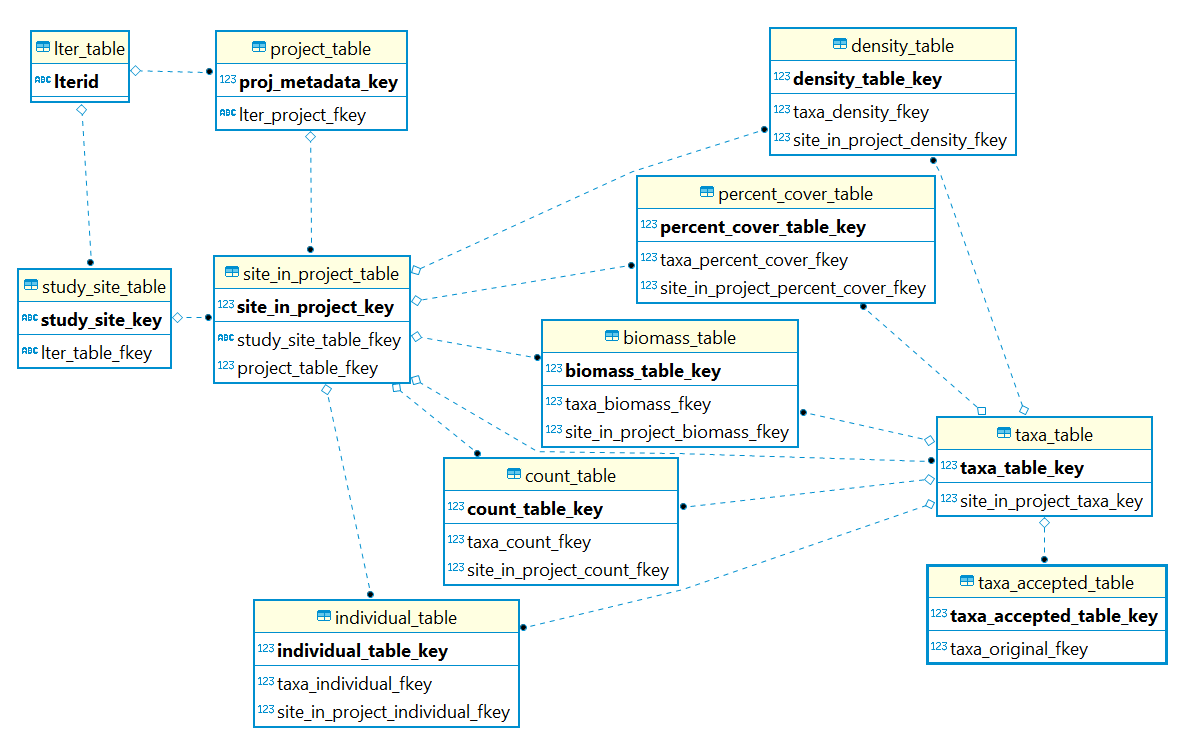
\includegraphics[scale=0.4]{simple_ERD}
    \caption{Simplified entity relationship diagram of the \texttt{popler} database. This figure shows table names, primary keys, and foreign keys of the \texttt{popler} database. It does not show, however, the other variable names contained in each table.}
    \label{Fig:simple_ERD}
  \end{center}
\end{figure}

\end{document}
